\documentclass[11pt]{amsart}
\usepackage{geometry}                % See geometry.pdf to learn the layout options. There are lots.
\geometry{letterpaper}                   % ... or a4paper or a5paper or ... 
%\geometry{landscape}                % Activate for for rotated page geometry
%\usepackage[parfill]{parskip}    % Activate to begin paragraphs with an empty line rather than an indent
\usepackage{graphicx}
\usepackage{amssymb}
\usepackage{epstopdf}
\usepackage{parskip}
\usepackage{setspace} 
\usepackage[options]{algorithm2e}
\setlength{\parindent}{15pt}

\DeclareGraphicsRule{.tif}{png}{.png}{`convert #1 `dirname #1`/`basename #1 .tif`.png}

\title{Data Preprocessing}
\author{The Author}
%\date{}                                           % Activate to display a given date or no date
\begin{document}
\begin{spacing}{1.1}

\maketitle
%\section{}
%\subsection{}
The DTW algorithm combined  with the  1 nearest neighbour classifier  is a memory based algorithm. Memory-based methods involve storing the entire training set in order to make predictions for future data points. They typically require a metric to be defined that measures the similarity of any two vectors in input space, and are generally fast to �train� but slow at making predictions for test data points. The time and computational complexity associated with such methods is even higher when the dimensionality of the data points is high. Intuitively speaking, DTW is a clustering algorithm that clusters similar patterns varying in time and speed. In high- dimensional spaces, however, the contrast between the nearest and furthest points gets increasingly smaller, making it difficult to construct meaningful cluster groups. To address this issue, data dimensionality methods are used at the  preprocessing stage.
 
Data-dimensionality reduction methodologies aim at mapping higher dimensional  patterns to low-dimensional spaces. There are presently two groups of techniques commonly used to address this issue:

\begin{itemize}
\item  Feature Selection 
\item Feature Extraction
\end{itemize}
 Feature selection techniques  involve selecting only a subset of attributes from the original data.  One of the most popular approaches to feature selection is  the exploratory data analysis(EDA). EDA is an approach to data analysis that postpones the usual assumptions about what kind of model the data follows with the more direct approach of allowing the data itself to reveal its underlying structure and models. The particular techniques employed in EDA are often quite simple, consisting of various techniques of:
 
 \begin{enumerate}
\item Plotting the raw data (such as data traces, histograms, histograms, probability plots, lag plots, block plots, and Youden plots.
\item Plotting simple statistics such as mean plots, standard deviation plots, box plots, and main effects plots of the raw data.
\item Positioning such plots so as to maximize our natural pattern-recognition abilities, such as using multiple plots per page.
 
Feature extraction processes on the other hand are concerned with  a range of techniques  that apply an appropriate functional mapping to the original attributes to extract new features.

\section{Feature Selection}
The computational and time complexity associated with the DTW algorithm is governed by the dimensionality of the time  series. One of the main goals of this project is to use unsupervised machine learning methods to discover important structural patterns that can be used to  cluster time series data sets suffering from  the curse of high dimensionality. Before applying models to the training and test data sets, the first step is to clean the data which in this problem domain mainly corresponds to feature selection. 

To remove redundant features, I have performed exploratory data analysis on the  isolated utterances. To get an idea about the structure of the data, I have studied the plots of the time series sequences along with performing auditory perception on the individual samples. From the visual and auditory analysis, I have made the following  observations:
\begin{itemize}
\item Long durations of silence occupy the beginning and end of each utterance.  An example is illustrated by figure 1. Figure 1 corresponds to a raw acoustic signal associated with a speaker belonging to the boy category uttering the digit `8'.  These durations of silence segments are considerably long compared to the interesting regions in the acoustic signal that actually contain information about the spoken digit .  Removing these silence segments not only  reduce the dimensionality of the time series but also results in minimal loss of information.
\item  Through auditory perception of numerous samples, I have discovered that  the recordings are highly distorted when played in matlab even when the data is scaled so that the sound is played as loud as possible without clipping. The distorted signal fails to provide any time auditory clue about  category of the speaker i.e whether the speaker belongs to \{ boy,girl, men,women\}  and the signal must be played multiple times  for its class to be correctly identified.
\end{itemize}
\begin{figure}[h!]
  \centering
   
     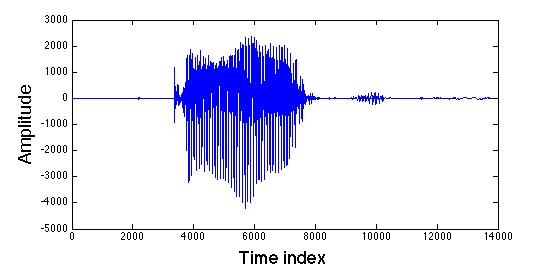
\includegraphics[scale=0.8]{Rawsample.jpg}
  \caption{`Raw 'signal}
  
\end{figure}
From  further experiments,  I have seen that if  I down-sample the utterances by $\frac{1}{2}$  which in other words means decreasing the sampling frequency by half, the resultant sampled signal is much clearer to understand. Sub-sampling  the utterances by half involves removing every other sample from the time series. This technique  keeps the global trend of the signal intact but results in the  loss of local information (see figure 2). From the observations made through auditory perception of the sampled signals, I have discovered that losing some \textbf{local information} actually cleans the signal in a manner that allows the listener to identity the speaker's category and the utterance's class with ease.

With the knowledge gained from exploratory data analysis, I have constructed a  signal filter that achieves dimensionality reduction by performing feature selection. The algorithm behind the filter is as follows:

\begin{algorithm}[H]
 \SetAlgoLined
 \KwData{rawSignal}
 \KwResult{output}
 threshold\;
 maxAmplitude= max(rawSignal)\\
 Adapt the threshold based on the value taken by the maximum amplitude\\
 signalSil\_R$\leftarrow$ removeSilence(rawSignal,threshold)\\
 output$\leftarrow$ downsample signalSil\_R by $\frac{1}{2}$\\
 end\\
  
 \caption{signal filter}
\end{algorithm}
 \begin {itemize}
 \item The algorithm removes all samples in the times series sequence whose magnitude is less than the threshold. The threshold used is an adaptive parameter. By using the information of the signal's maximum amplitude the algorithm sets the threshold accordingly. It raises the threshold for signals corresponding to speakers having a loud and deep voice is higher  and lowers the threshold for signals corresponding to speakers having as gentle and low voice.
 \end{itemize}   
  Figure 2 shows the raw acoustic signal corresponding to the utterances of the digit '5' alongside with the version that has its dimensionality reduced by the filter discussed above. From the comparison of the plots, it can be observed that the filter preserves the interesting patterns associated with the utterance while succeeding in reducing the dimensionality of the data.    
  \end{itemize} 
 \begin{figure}[h!]
  \centering
   
     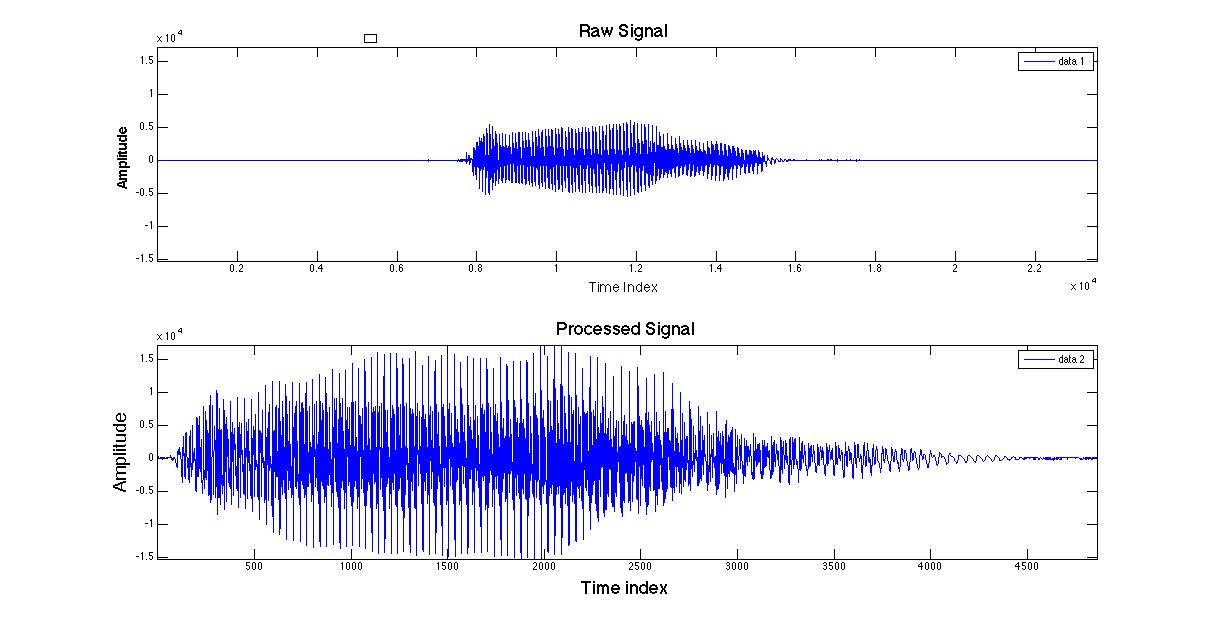
\includegraphics[scale=0.4]{Feature_selection.jpg}
  \caption{`Raw' Signal Vs `Cleaned' Signal }
  
\end{figure}
 

 

\end{spacing}
\end{document}  